% ============================================================
%  Chapter 4: Evaluation
% ============================================================

\chapter{Evaluation}
\label{chap:results}

% ============================================================
%  Section 4.1 — Headline reproduction result
% ============================================================
\section{Headline reproduction result}
\label{sec:headline}

The headline TFPnP result comes from \texttt{run\_04\_pat\_250\_e80}, where the policy is trained on 250 LIDC patients over 80 epochs, using the natural-image DRUNet as the denoiser prior and PSNR as the reward function. All evaluations use the full LIDC-IDRI test set (389 images) at three sinogram noise levels (5\%, 7.5\%, 10\%). The full experiment configuration is documented in~\Cref{sec:tfpnp-policy}.

Six reconstruction methods are compared, including classical baselines (FBP and TV), the denoiser applied directly to the FBP reconstruction (DRUNet), an end-to-end learned network (FBPConvNet), and two hyperparameters, and the TFPnP reproduction with the learned policy). \Cref{tab:headline_full} reports mean PSNR, SSIM, and HaarPSI at each noise level.

The reproduction confirms the paper's central claim, with TFPnP achieving \textbf{27.27\,dB} PSNR at 5\% noise, a $+2.96$\,dB improvement over Fixed PnP-ADMM. Perceptual metrics (SSIM $= 0.691$, HaarPSI $= 0.485$) improve similarly over Fixed PnP-ADMM ($0.499$ and $0.405$), confirming that the learned policy provides measurable value across all metrics.

One finding departs from the paper's ranking. FBPConvNet reaches $28.58$\,dB at 5\% noise, $+1.31$\,dB above TFPnP, whereas~\citet{Wei2022TFPnP} report TFPnP ahead of FBPconv by $+1.50$\,dB. The ranking inverts by 10\% noise (\Cref{sec:cross-noise}), and the underlying causes are analysed in~\Cref{sec:why-fbpconvnet}. \Cref{fig:reconstruction_gallery} shows a visual comparison of the best, median, and worst reconstructions.

% ------------------------------------------------------------
%  Table 4.1: Full test set × 3 noise levels × 6 methods × 3 metrics
% ------------------------------------------------------------
\begin{table}[H]
    \centering
    \footnotesize
    \caption{Reconstruction quality on the LIDC-IDRI test set (389 images).
    Best in \textbf{bold}, second-best \underline{underlined}.}
    \label{tab:headline_full}
    \begin{tabular}{lccc ccc ccc}
        \toprule
        & \multicolumn{3}{c}{\textbf{5\% noise}}
        & \multicolumn{3}{c}{\textbf{7.5\% noise}}
        & \multicolumn{3}{c}{\textbf{10\% noise}} \\
        \cmidrule(lr){2-4} \cmidrule(lr){5-7} \cmidrule(lr){8-10}
        Method & PSNR & SSIM & HaarPSI & PSNR & SSIM & HaarPSI & PSNR & SSIM & HaarPSI \\
        \midrule
        FBP                    & 14.56 & 0.075 & 0.233 & 13.65 & 0.058 & 0.223 & 13.22 & 0.052 & 0.216 \\
        TV                     & 19.67 & 0.288 & 0.390 & 18.35 & 0.271 & 0.348 & 17.50 & 0.248 & 0.315 \\
        DRUNet ($\sigma{=}10$) & 21.80 & 0.455 & 0.384 & 19.50 & 0.418 & 0.312 & 18.16 & 0.391 & 0.245 \\
        FBPConvNet             & \textbf{28.58} & \textbf{0.726} & \textbf{0.556} & \textbf{27.14} & 0.619 & \textbf{0.490} & 24.73 & 0.463 & 0.385 \\
        Fixed PnP-ADMM         & 24.31 & 0.499 & 0.405 & 22.42 & 0.376 & 0.336 & 21.50 & 0.340 & 0.290 \\
        TFPnP (Ours)           & \underline{27.27} & \underline{0.691} & \underline{0.485} & \underline{26.58} & \textbf{0.681} & \underline{0.443} & \textbf{26.10} & \textbf{0.676} & \textbf{0.413} \\
        \bottomrule
    \end{tabular}
\end{table}

% ------------------------------------------------------------
%  Figure 4.1: Contact-sheet reconstruction gallery
% ------------------------------------------------------------
\begin{figure}[H]
    \centering
    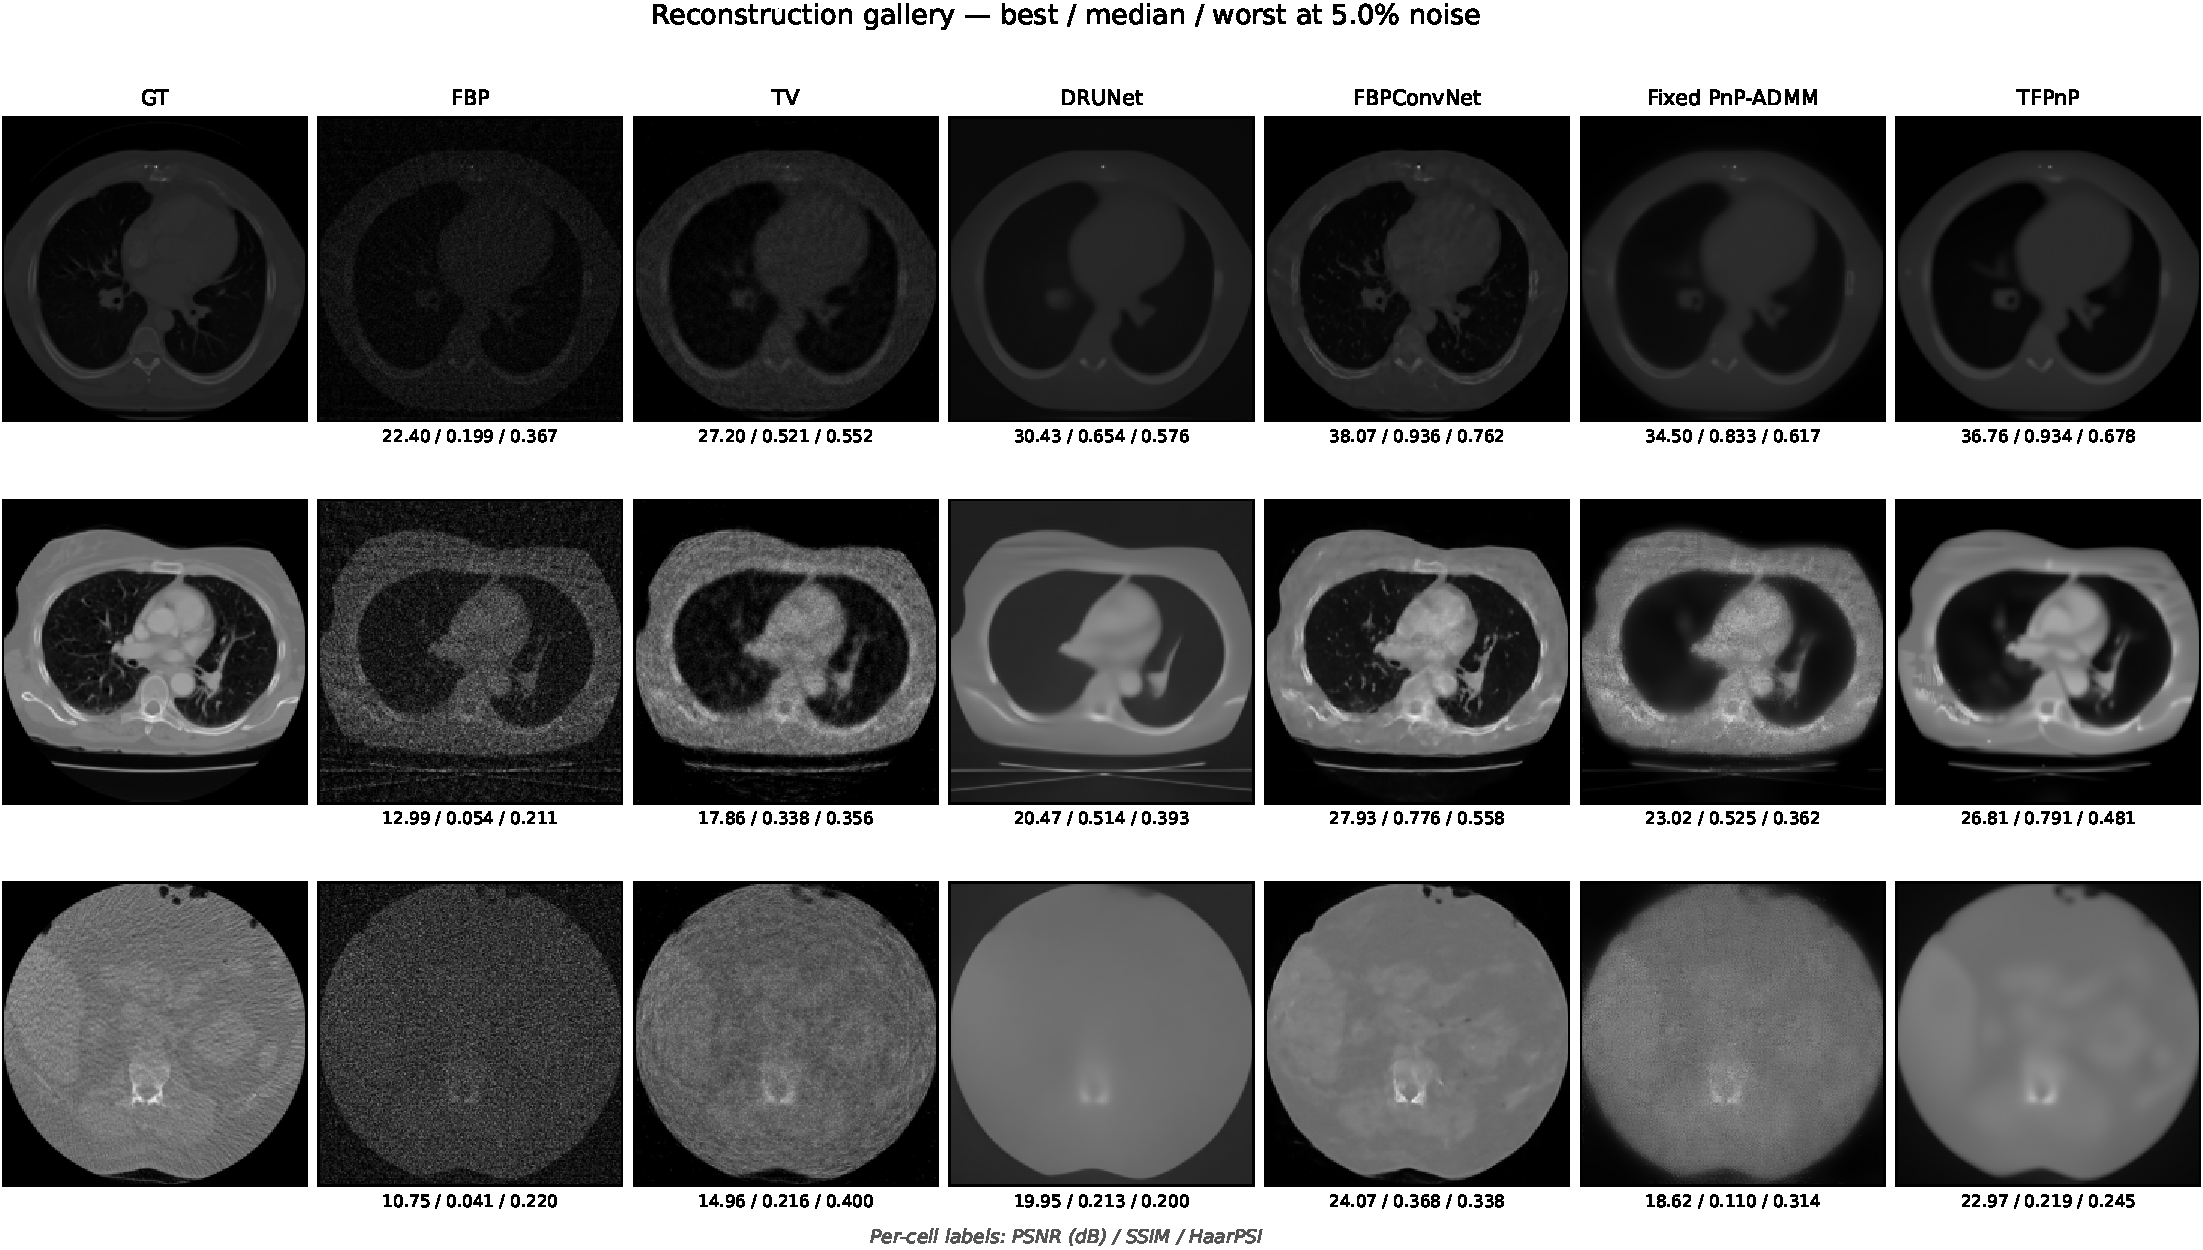
\includegraphics[width=\linewidth]{../figures/run_04_pat_250_e80/gallery.pdf}
    \caption{Reconstruction gallery for \texttt{run\_04} at 5\% noise.
    Rows: best, median, and worst test images by TFPnP PSNR.
    Per-cell labels give PSNR, SSIM, and HaarPSI.}
    \label{fig:reconstruction_gallery}
\end{figure}

% ============================================================
%  Section 4.2 — Cross-noise behaviour
% ============================================================
\section{Cross-noise behaviour}
\label{sec:cross-noise}

TFPnP's practical value depends not only on its performance at the training noise level but also on how well it generalises across the noise range seen at inference. \Cref{fig:metrics_vs_noise} traces mean PSNR, SSIM, and HaarPSI as sinogram noise increases from 5\% to 10\%. TFPnP degrades gracefully, with PSNR dropping only $-1.17$\,dB (from $27.27$ to $26.10$) and SSIM remains effectively flat ($0.691$ to $0.676$). This robustness reflects the strength of the plug-and-play iterative approach, since the policy can adapt the denoising strength
and penalty parameter to different noise levels, rather than producing a single fixed reconstruction.

By contrast, FBPConvNet degrades steeply across the same range ($-3.85$\,dB PSNR, SSIM from $0.726$ to $0.463$), and TFPnP overtakes it on all three metrics at $10\%$ noise. This is partly due to a methodological difference, as our FBPConvNet was trained at a fixed 5\% noise level (\Cref{sec:baselines}) and extrapolates at higher noise. However, the crossover on perceptual metrics at $10\%$ suggests that the iterative structure of TFPnP provides a robustness that training-distribution matches alone would not explain, and is analysed further in~\Cref{sec:why-fbpconvnet}.

% ------------------------------------------------------------
%  Figure 4.2: Metrics vs noise level line plot
% ------------------------------------------------------------
\begin{figure}[H]
    \centering
    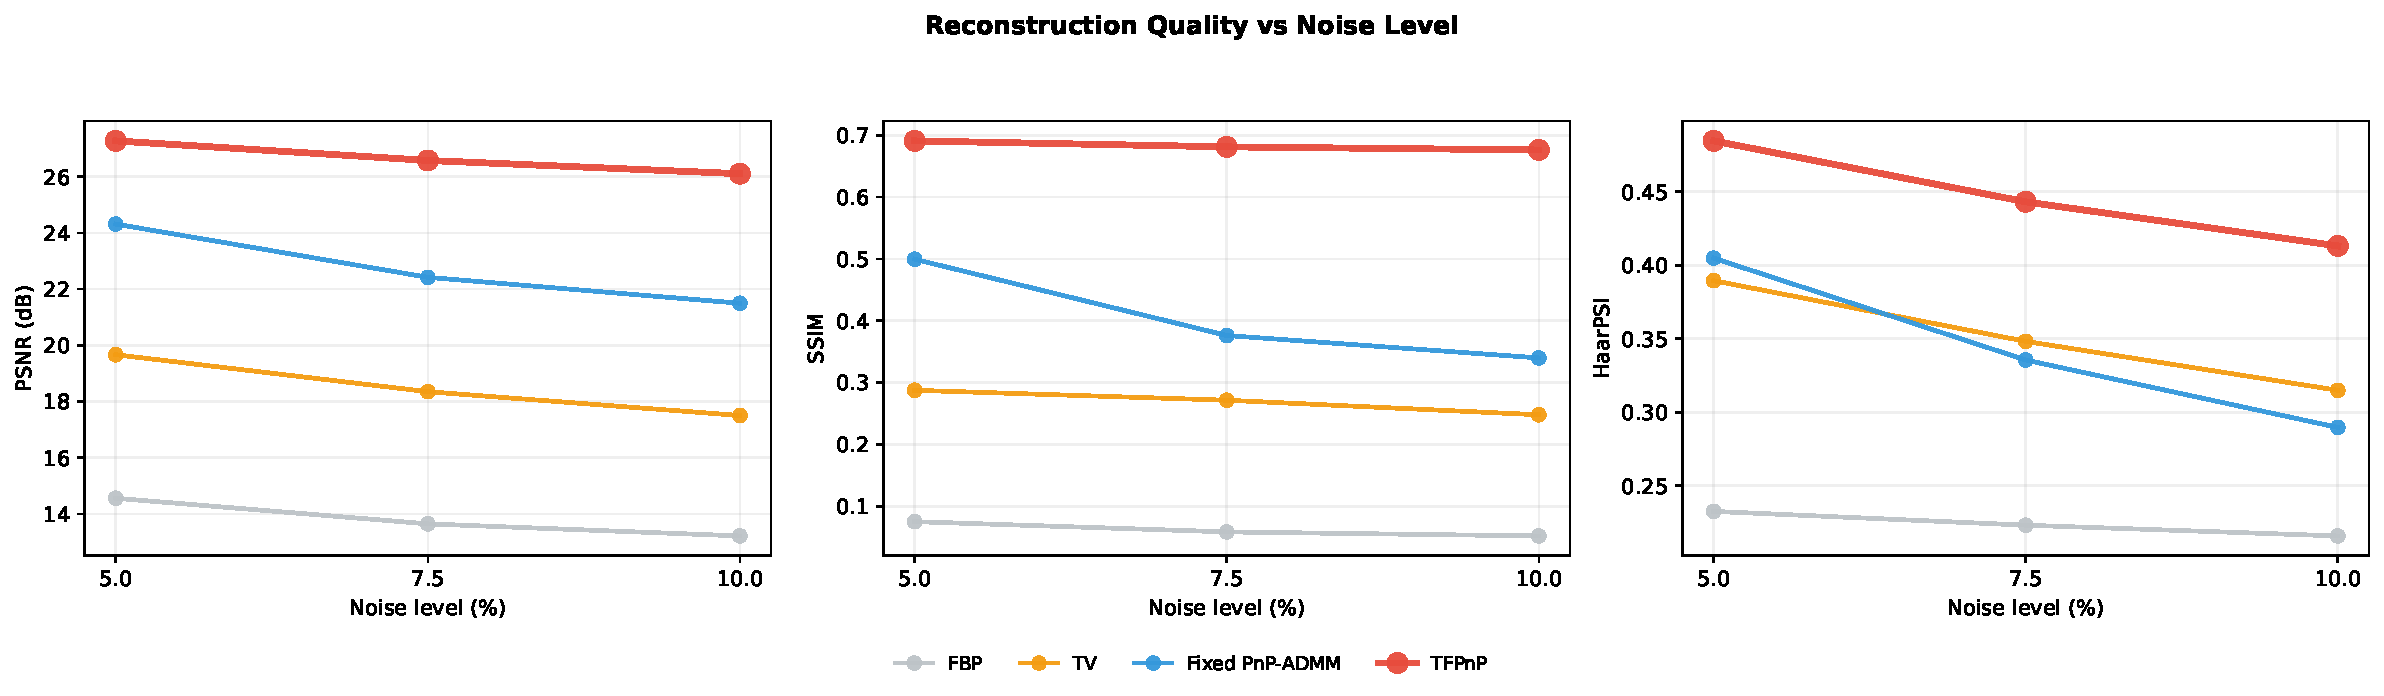
\includegraphics[width=\linewidth]{../figures/run_04_pat_250_e80/metrics_vs_noise.pdf}
    \caption{Mean PSNR, SSIM, and HaarPSI vs sinogram noise level.
    TFPnP overtakes FBPConvNet on all three metrics at 10\% noise.}
    \label{fig:metrics_vs_noise}
\end{figure}

% ============================================================
%  Section 4.3 — Per-image variance
% ============================================================
\section{Per-image variance}
\label{sec:per-image}

Averaging hides per-image variability. \Cref{fig:per_image_psnr} shows TFPnP's three largest wins and losses over the next-best non-TFPnP method at $5\%$ noise, ranked by per-image PSNR delta. TFPnP's wins tend to occur on homogeneous slices with large uniform regions, while losses occur on complex slices with high-frequency detail such as multiple small nodules or intricate anatomy that doesn't contain the lungs. Per-image variability (standard deviations of $\sim 1.5$--$2$\,dB across all methods) means no method dominates uniformly, and reconstructions of comparable quality across methods are common. This is consistent with the general finding that PnP and end-to-end methods have complementary strengths, with neither uniformly outperforming the other.

% ------------------------------------------------------------
%  Figure 4.3: Per-image PSNR bar chart
% ------------------------------------------------------------
\begin{figure}[H]
    \centering
    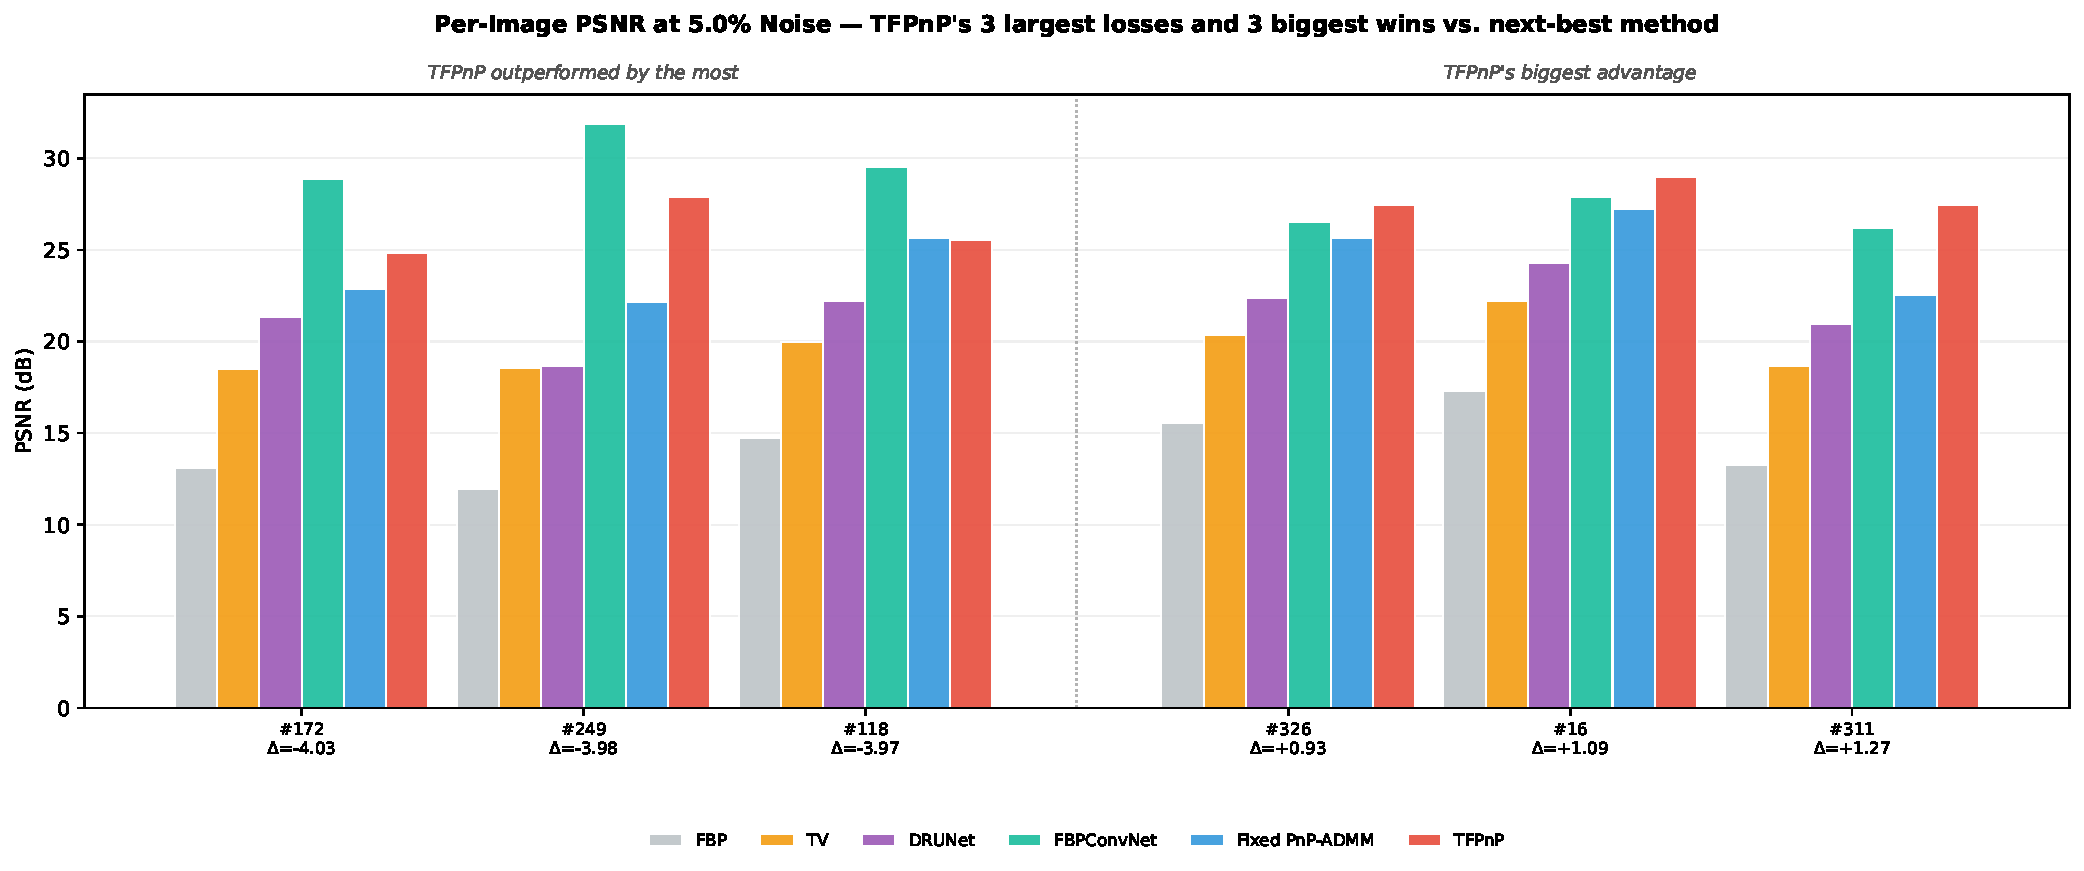
\includegraphics[width=\linewidth]{../figures/run_04_pat_250_e80/per_image_psnr.pdf}
    \caption{Per-image PSNR at 5\% noise. TFPnP's three largest wins
    (left) and losses (right) versus the next-best non-TFPnP method.
    Homogeneous slices favour TFPnP, complex ones favour FBPConvNet.}
    \label{fig:per_image_psnr}
\end{figure}

% ============================================================
%  Section 4.4 — Hyperparameter calibration sweeps
% ============================================================
\section{Hyperparameter calibration sweeps}
\label{sec:calibration}

The Fixed PnP-ADMM baseline uses hand-calibrated $\sigma = 1.5$ and $\mu = 20$ values for the natural-image DRUNet, identified through sensitivity sweeps during notebook development. When the denoiser is swapped for the CT-trained DRUNet developed in~\Cref{sec:ct-drunet}, this calibration is no longer valid, and~\Cref{fig:sigma_sweep_natural} and~\Cref{fig:sigma_sweep_ct} present calibration sweeps for both denoisers. The CT-trained DRUNet peaks at $\sigma = 8.0$ in the wrapper's units; the interpretation of this apparent shift is revisited in~\Cref{sec:corrections}. The corresponding $\mu$ sweep at $\sigma = 8$ (see~\Cref{fig:mu_sweep_ct}) reveals a peak at $\mu = 10$, half the natural-DRUNet value.

Two limitations of these sweeps are worth noting. First, they were performed on a single representative slice at 5\% noise, and a broader sweep across the validation set was intended but could not be completed within the available compute budget. Second, the sweep grids used $\sigma \in [1, 25]$ and $\mu \in [5, 50]$, but a finer grid around the peak could refine the calibration further.

% ------------------------------------------------------------
%  Figure 4.4a: σ sensitivity sweep — natural DRUNet
% ------------------------------------------------------------
\begin{figure}[H]
    \centering
    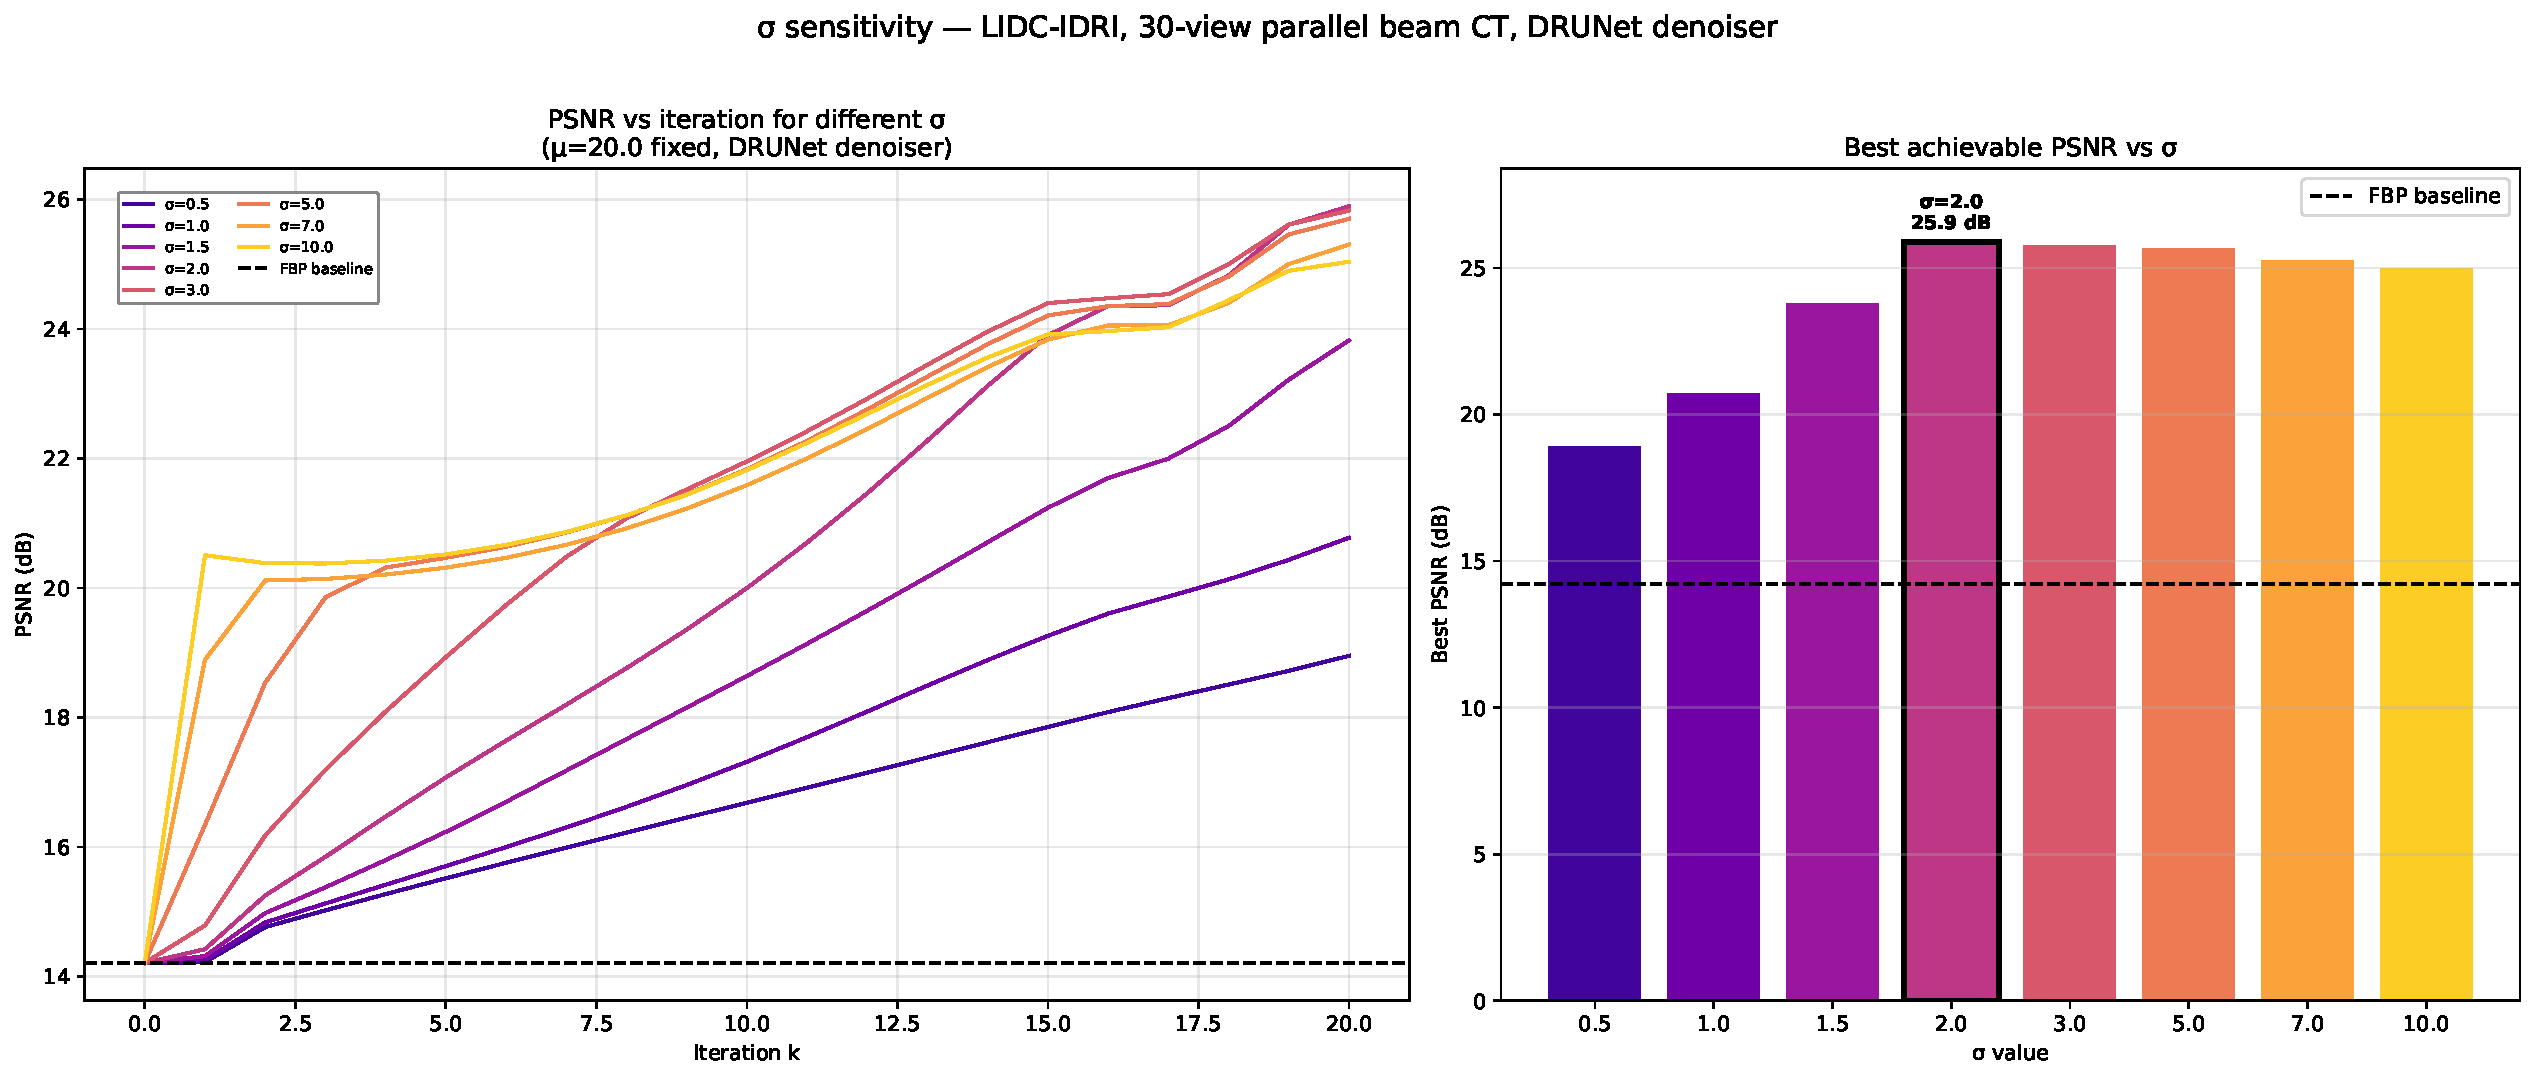
\includegraphics[width=\linewidth]{../figures/05/07_sigma_sensitivity.pdf}
    \caption{$\sigma$ sensitivity for natural-image DRUNet within Fixed
    PnP-ADMM at 5\% noise. Peak at $\sigma = 1.5$.}
    \label{fig:sigma_sweep_natural}
\end{figure}

% ------------------------------------------------------------
%  Figure 4.4b: σ sensitivity sweep — CT DRUNet
% ------------------------------------------------------------
\begin{figure}[H]
    \centering
    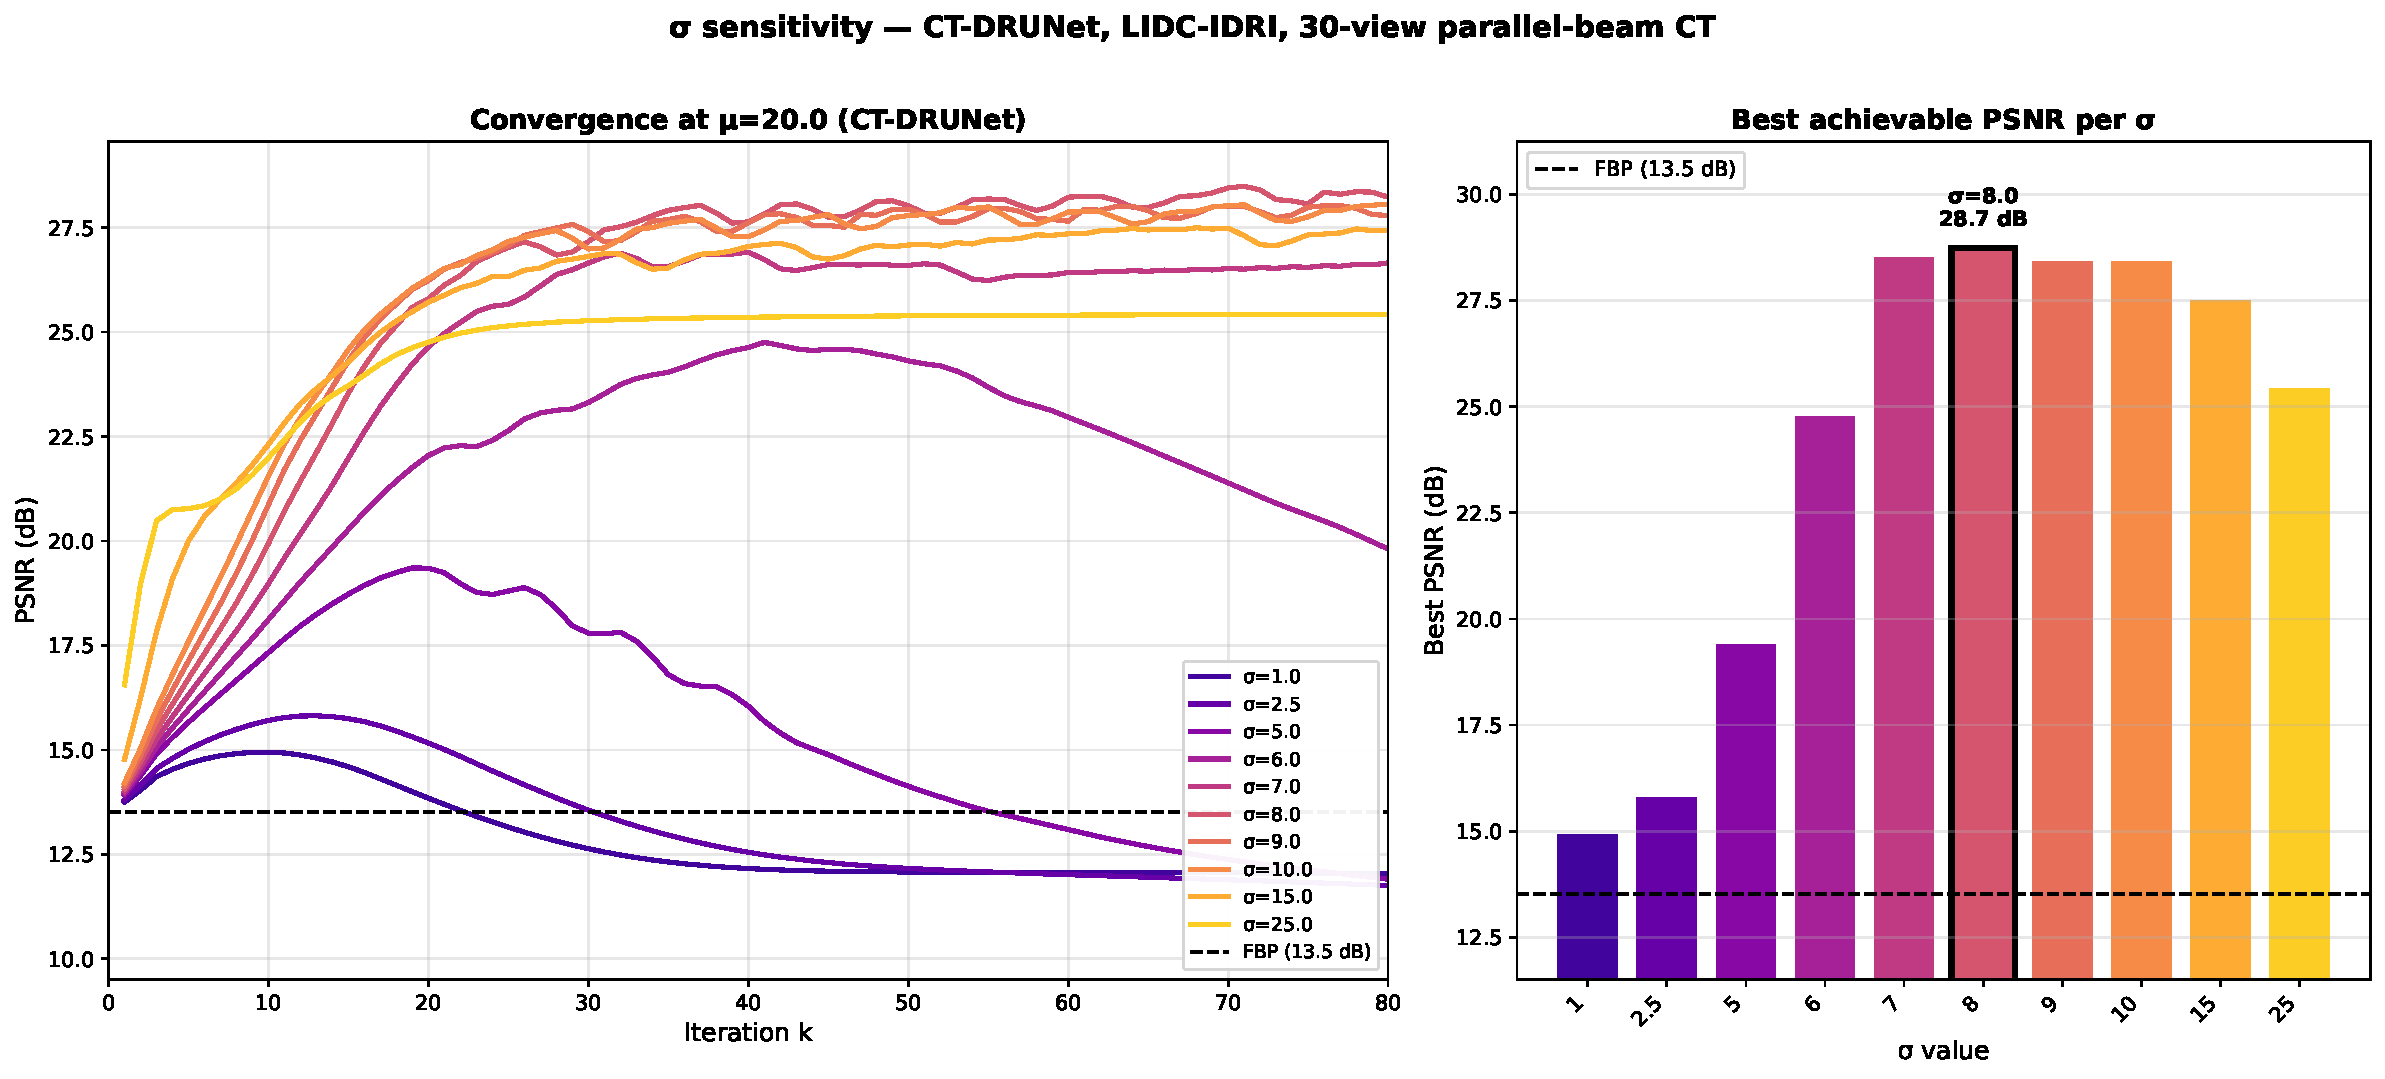
\includegraphics[width=\linewidth]{../figures/12/06_sigma_sensitivity_ctdrunet.pdf}
    \caption{$\sigma$ sensitivity for CT-trained DRUNet within Fixed PnP-ADMM
    at 5\% noise. Peak at $\sigma = 8.0$.}
    \label{fig:sigma_sweep_ct}
\end{figure}

% ------------------------------------------------------------
%  Figure 4.4c: µ sensitivity sweep — CT DRUNet at σ=8
% ------------------------------------------------------------
\begin{figure}[H]
    \centering
    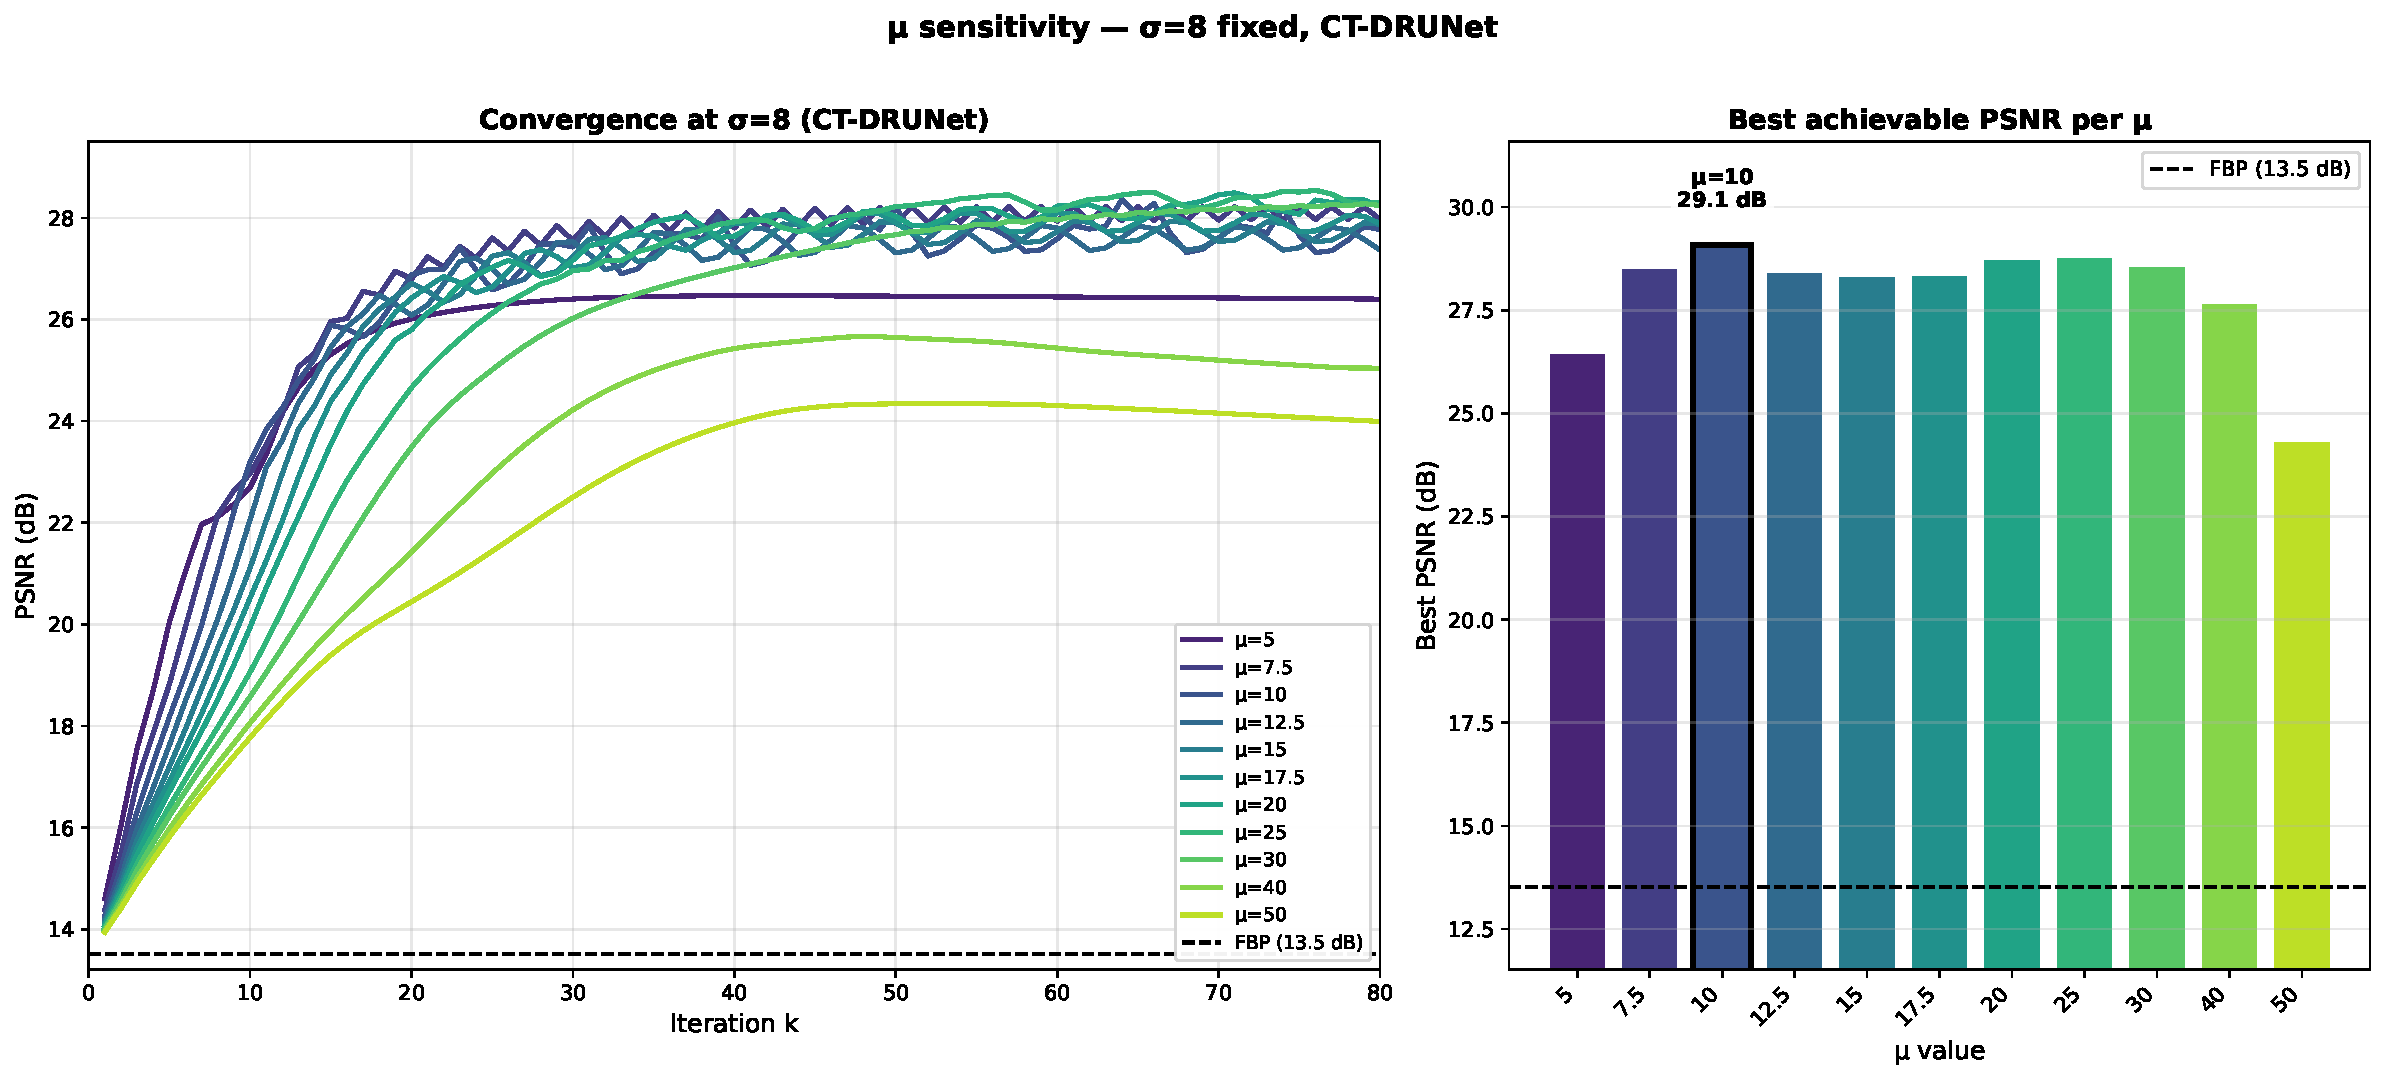
\includegraphics[width=\linewidth]{../figures/12/07_mu_sensitivity_ctdrunet.pdf}
    \caption{$\mu$ sensitivity for CT-trained DRUNet at $\sigma = 8$. Peak
    at $\mu = 10$.}
    \label{fig:mu_sweep_ct}
\end{figure}

% ============================================================
%  Section 4.5 — In-domain denoiser experiment
% ============================================================
\section{In-domain denoiser experiment}
\label{sec:in-domain}

With the CT-trained DRUNet calibrated to its own operating point ($\sigma = 8$, $\mu = 10$), a paired comparison of Fixed PnP-ADMM using each denoiser at its respective optimum was performed on the full 389-image test set (\Cref{tab:fixed_pnp_ct_vs_natural}). The CT-DRUNet outperforms the natural-image DRUNet at every noise level, and the advantage grows with noise, from $+0.71$\,dB at 5\% to $+1.98$\,dB at 10\%. SSIM improvements follow the same trend, from $+0.037$ to $+0.090$.

The advantage grows with noise; its interpretation is discussed in~\Cref{sec:in-domain-gap}. \Cref{fig:fixed_pnp_optimum_comparison} shows a visual comparison at all three noise levels.

This comparison uses Fixed PnP-ADMM rather than TFPnP with the learned policy, as retraining the policy against the CT denoiser (\Cref{sec:run11}) encountered training instability that could not be resolved before a CSD3 cluster outage.

% ------------------------------------------------------------
%  Table 4.3: Fixed PnP-ADMM — natural vs CT-DRUNet at each optimum
% ------------------------------------------------------------
\begin{table}[H]
    \centering
    \footnotesize
    \caption{Fixed PnP-ADMM at each denoiser's calibrated optimum.}
    \label{tab:fixed_pnp_ct_vs_natural}
    \begin{tabular}{lcc cc cc cc}
        \toprule
        & \multicolumn{2}{c}{\textbf{5\% noise}}
        & \multicolumn{2}{c}{\textbf{7.5\% noise}}
        & \multicolumn{2}{c}{\textbf{10\% noise}}
        & \multicolumn{2}{c}{\textbf{Advantage}} \\
        \cmidrule(lr){2-3} \cmidrule(lr){4-5} \cmidrule(lr){6-7} \cmidrule(lr){8-9}
        Denoiser        & PSNR  & SSIM  & PSNR  & SSIM  & PSNR  & SSIM  & PSNR  & SSIM  \\
        \midrule
        Natural DRUNet ($\sigma{=}1.5$) & 28.06 & 0.752 & 26.52 & 0.695 & 25.41 & 0.652 & -- & -- \\
        CT DRUNet ($\sigma{=}8$)       & \textbf{28.77} & \textbf{0.789} & \textbf{27.91} & \textbf{0.768} & \textbf{27.39} & \textbf{0.742} & $+0.71$ to $+1.98$ & $+0.037$ to $+0.090$ \\
        \bottomrule
    \end{tabular}
\end{table}

% ------------------------------------------------------------
%  Figure 4.6: Fixed PnP-ADMM at optimum comparison
% ------------------------------------------------------------
\begin{figure}[H]
    \centering
    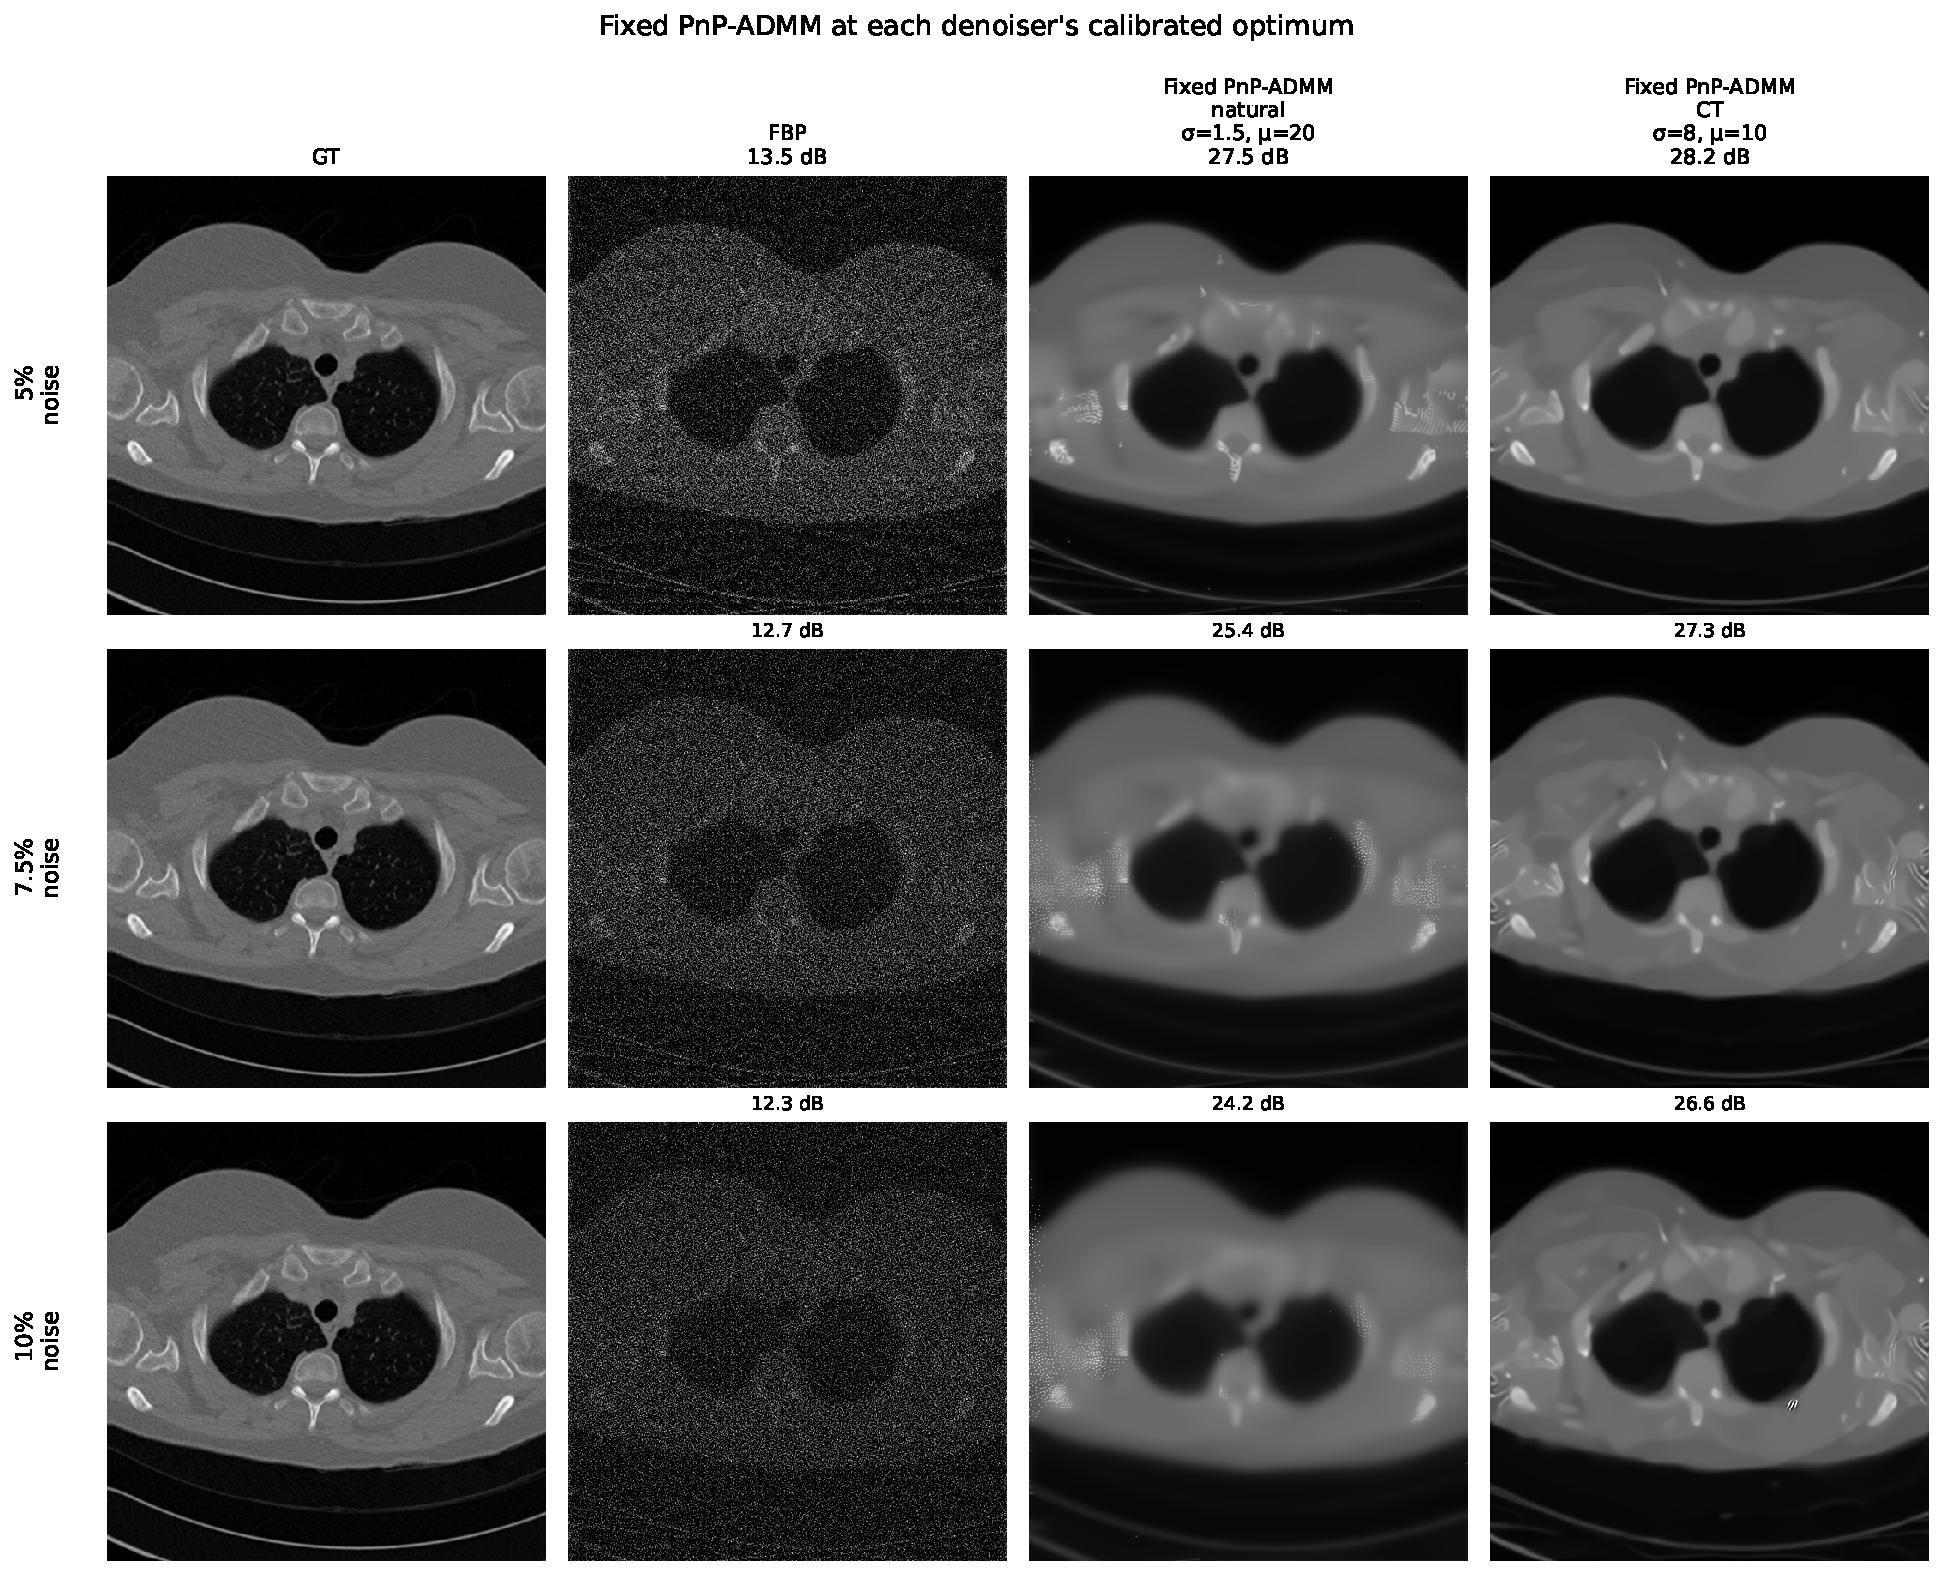
\includegraphics[width=\linewidth]{../figures/12/08_fixed_pnp_optimum_comparison.pdf}
    \caption{Fixed PnP-ADMM with denoisers at their calibrated optimum, at 5\%, 7.5\%, and 10\% noise.}
    \label{fig:fixed_pnp_optimum_comparison}
\end{figure}

% ============================================================
%  Section 4.6 — TFPnP policy retrain with CT-DRUNet
% ============================================================
\section{TFPnP policy retrain with CT-DRUNet}
\label{sec:run11}

The natural next step is retraining the TFPnP policy against the CT-DRUNet, with a widened $\sigma$ action range $[1, 15]$ to cover the new optimum and a narrowed $\mu$ range $[5, 50]$ chosen to keep the ADMM balance stable at the higher $\sigma$ values. This run (\texttt{run\_11}) underperformed \texttt{run\_04}, reaching only $26.51$\,dB at 5\% noise, well below \texttt{run\_04}'s $27.27$\,dB and below even the Fixed PnP-ADMM baseline with CT-DRUNet at $28.77$\,dB (\Cref{sec:in-domain}).

\Cref{fig:run11_training_curves} shows the diagnostic training curves. Around policy update step 15{,}000, the critic loss explodes to $10^{19}$-scale magnitudes, the policy's mean $\sigma$ output drifts from $\sim 14$ to $\sim 9$, and both training and validation PSNR collapse from their earlier trajectory. The best checkpoint is saved from epoch 1, indicating no improvements were made. Since both the $\sigma$ and $\mu$ ranges were changed simultaneously, the failure cannot be attributed to either alone, but the drift in the policy's mean $\sigma$ output suggests the widened action space is the more likely cause. A third factor cannot be excluded. Our value network omits the weight normalisation and TReLU that Table~1 of~\citet{Wei2022TFPnP} specifies for the critic (\Cref{sec:tfpnp-policy}), and both are adopted in their source papers for their stabilising effect on training. Whether the divergence follows from the widened action range, from this architectural omission, or from both, could not be separated at the time. A post-hoc diagnosis identifying a further, more fundamental cause is given in~\Cref{sec:corrections}.

% ------------------------------------------------------------
%  Figure 4.5: run_11 training curves
% ------------------------------------------------------------
\begin{figure}[H]
    \centering
    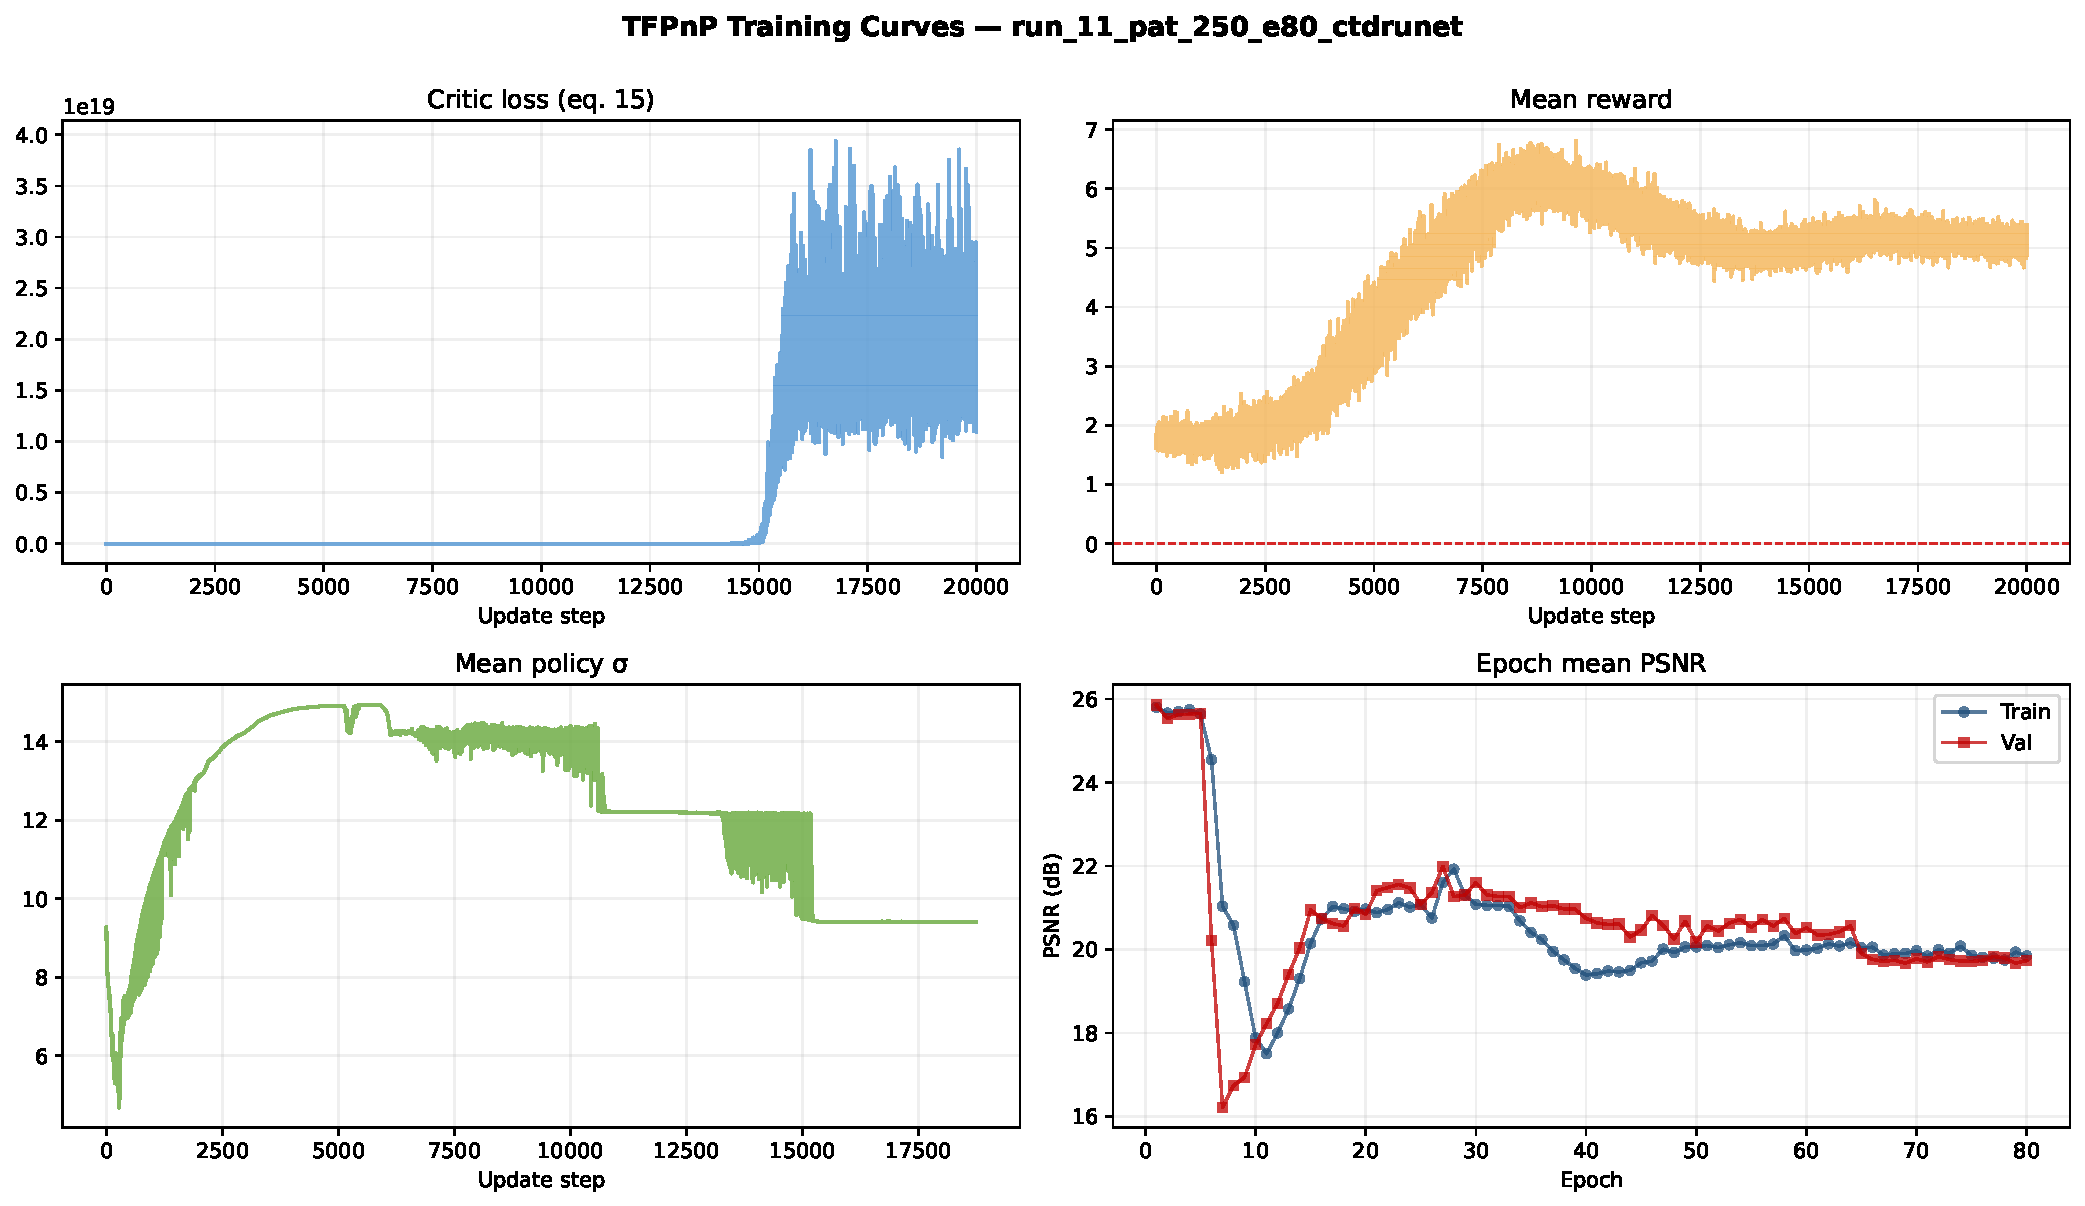
\includegraphics[width=\linewidth]{../figures/run_11_pat_250_e80_ctdrunet/training_curves.pdf}
    \caption{Training curves for \texttt{run\_11}.}
    \label{fig:run11_training_curves}
\end{figure}

% ============================================================
%  Section 4.7 — Reward shaping ablations
% ============================================================
\section{Reward shaping ablations}
\label{sec:reward-shaping}

Four variant runs were carried out to test whether alternative reward signals could improve metric-specific performance, motivated by the finding of~\citet{breger2025study} that PSNR correlates poorly with perceived image quality in medical imaging, raising the question of whether an RL policy rewarded on different metrics would produce better reconstructions than one trained on PSNR alone. The study is an extension undertaken in addition to the reproduction, rather than a component of~\citet{Wei2022TFPnP}'s original methodology, and results are summarised in~\Cref{tab:reward_shaping}.

The reward coefficients compensate for the difference in numeric scale between metrics. A typical per-step $\Delta\text{PSNR}$ is on the order of $0.1$--$1.0$, whereas $\Delta\text{SSIM}$ and $\Delta\text{HaarPSI}$ are on the order of $0.001$--$0.01$, so without scaling, the they would be roughly $100\times$ smaller than the PSNR term and contribute negligibly to the policy gradient. The mixed rewards (\texttt{run\_07}, \texttt{run\_08}) therefore use $\alpha = 5$ to bring the perceptual term to a comparable order of magnitude as $\Delta\text{PSNR}$, and the pure-replacement rewards (\texttt{run\_09}, \texttt{run\_10}) use $\alpha = 50$ so the overall reward magnitude remains comparable to \texttt{run\_04}'s pure-PSNR reward.

The SSIM-only reward (\texttt{run\_09}) achieves the highest PSNR and HaarPSI among all runs, and the mixed PSNR/SSIM reward (\texttt{run\_07}) wins on SSIM specifically. In contrast, both HaarPSI-based rewards (\texttt{run\_08} PSNR/HaarPSI, \texttt{run\_10} HaarPSI only) underperform across all metrics. Given only a single training seed per configuration, some of this variation likely reflects RL training stochasticity rather than the differences between reward functions, so the PSNR reward chosen for \texttt{run\_04} remains a defensible default for direct comparison to the paper.

% ------------------------------------------------------------
%  Table 4.4: Reward-shaping ablation summary (runs 07-10)
% ------------------------------------------------------------
\begin{table}[H]
    \centering
    \footnotesize
    \caption{Reward-shaping ablation at 5\% noise. Best values in \textbf{bold}.}
    \label{tab:reward_shaping}
    \begin{tabular}{llccc}
        \toprule
        Run & Reward function & PSNR & SSIM & HaarPSI \\
        \midrule
        \texttt{run\_04} & PSNR (main)     & 27.27          & 0.691          & 0.485          \\
        \texttt{run\_07} & PSNR + SSIM     & 27.18          & \textbf{0.707} & 0.481          \\
        \texttt{run\_08} & PSNR + HaarPSI  & 26.47          & 0.640          & 0.437          \\
        \texttt{run\_09} & SSIM only       & \textbf{27.32} & 0.695          & \textbf{0.489} \\
        \texttt{run\_10} & HaarPSI only    & 26.76          & 0.658          & 0.460          \\
        \bottomrule
    \end{tabular}
\end{table}
